% $Header$

\documentclass{beamer}


\mode<presentation>
{
  \usetheme{Boadilla}
  % or ...

  \usecolortheme{seahorse}
  \useinnertheme{rectangles}
  \useoutertheme[hooks]{tree}
  \setbeamercovered{transparent}
  
  % or whatever (possibly just delete it)
}

\usepackage{bm}
\usepackage[english]{babel}
% or whatever


\usepackage[latin1]{inputenc}
% or whatever
\usepackage{graphicx}
\usepackage{tikz}
\usepackage{pgfplots}
\usepackage{graphicx} 
\usepackage{animate}
\usepackage{movie15}
\usepackage{listings}
\usepackage[super]{nth}

\usepackage[T1]{fontenc}
% Or whatever. Note that the encoding and the font should match. If T1
% does not look nice, try deleting the line with the fontenc.



\usepackage{amsmath}
\usepackage{amsthm}
\usepackage{amssymb}

\usepackage{listings}
\usepackage{xcolor}

\definecolor{codegreen}{rgb}{0,0.6,0}
\definecolor{codegray}{rgb}{0.5,0.5,0.5}
\definecolor{codepurple}{rgb}{0.58,0,0.82}
\definecolor{backcolour}{rgb}{0.95,0.95,0.92}

\lstdefinestyle{mystyle}{
    backgroundcolor=\color{backcolour},   
    commentstyle=\color{codegreen},
    keywordstyle=\color{magenta},
    numberstyle=\tiny\color{codegray},
    stringstyle=\color{codepurple},
    basicstyle=\ttfamily\footnotesize,
    breakatwhitespace=false,         
    breaklines=true,                 
    captionpos=b,                    
    keepspaces=true,                 
    numbers=left,                    
    numbersep=5pt,                  
    showspaces=false,                
    showstringspaces=false,
    showtabs=false,                  
    tabsize=2
}

\lstset{style=mystyle}


% \title[\text{Computational Geometry}] % (optional, use only with long paper titles)
% {CS 424: Joy of Theoretical Computer Science}

\title[Geometric Algorithms: Convex Hull]{Geometric Algorithms -- The Convex Hull Problem in 2 \& 3 Dimensions}

\author[Rehman, Ali, Ozair] % (optional, use only with lots of authors)
{Rehman, M. Usaid \and Ali, Syed Anus \and Ozair, Faraz}

\institute{Habib University} % (optional, but mostly needed)
\date{\today} % (optional, should be abbreviation of conference name)

\pgfdeclareimage[height=0.5cm]{university-logo}{logo.jpg}
\logo{\pgfuseimage{university-logo}}

%Delete this, if you do not want the table of contents to pop up at
% the beginning of each subsection:

% \AtBeginSubsection[]
% {
%   \begin{frame}<beamer>{Outline}
%     \tableofcontents[currentsection,currentsubsection]
%   \end{frame}
% }
% \beamerdefaultoverlayspecification{<+->}


\makeatletter
\setbeamertemplate{footline}
{
  \leavevmode%
  \hbox{%
  \begin{beamercolorbox}[wd=.333333\paperwidth,ht=2.25ex,dp=1ex,center]{author in head/foot}%
    \usebeamerfont{author in head/foot}\insertshortauthor%~~\beamer@ifempty{\insertshortinstitute}{}{(\insertshortinstitute)}
  \end{beamercolorbox}%
  \begin{beamercolorbox}[wd=.333333\paperwidth,ht=2.25ex,dp=1ex,center]{title in head/foot}%
    \usebeamerfont{title in head/foot}\insertshorttitle
  \end{beamercolorbox}%
  \begin{beamercolorbox}[wd=.333333\paperwidth,ht=2.25ex,dp=1ex,right]{date in head/foot}%
    \usebeamerfont{date in head/foot}\insertshortdate{}\hspace*{2em}
    \insertframenumber{} / \inserttotalframenumber\hspace*{2ex} 
  \end{beamercolorbox}}%
  \vskip0pt%
}
\makeatother

\begin{document}

\begin{frame}
  \titlepage
\end{frame}

\begin{frame}{Outline}
  \tableofcontents%[pausesections]
  % You might wish to add the option [pausesections]
\end{frame}


\section{Introduction to Computational Geometry}

\subsection{Overview}
\begin{frame}
  \frametitle{The Paradigm of Computational Geometry}
\end{frame}

\subsection{History \& Areas of Application}
\begin{frame}
  \frametitle{A Brief History \& Timeline}
\end{frame}

\begin{frame}{Famous Problems \& Their Applications}
    
\end{frame}

\section{Geometric Preliminaries}
\subsection{Definitions \& Notation}
\begin{frame}
  \frametitle{Basics of Euclidean Geometry}
\end{frame}

\section{The Convex Hull Problem}
\subsection{Introduction}

\begin{frame}{What is a Convex Hull?}
    \begin{itemize}
        \item A \emph{convex set} is a subset of Euclidean space where given any two points in the set,  the set contains the whole line segment joining them.
        \item A  \emph{convex hull} of a shape is the smallest convex set containing the shape. 
        \item The convex hull can also be defined as the intersection of all convex
        sets of a given subset of Euclidean space. 
    \end{itemize}
    \begin{figure}
        \centering
        \begin{tikzpicture}
        \draw[rotate=-45,fill=gray!30] (0,0) ellipse (29pt and 44pt);
        \node[circle, fill=black,inner sep=0pt,minimum size=5pt] (A) at (0.5,0.75) {};
        \node[circle, fill=black,inner sep=0pt,minimum size=5pt] (B) at (-0.25,-0.5) {};
        \draw[thick] (A) -- (B) {};
        \end{tikzpicture}
        \caption{A convex set}
        \label{convex}
    \end{figure}
\end{frame}

\begin{frame}[t]{Formal Definitions}
    \begin{definition}[Convex Set]
        Given $k$ distinct points $p_1, p_2, \dots, p_k$ in $E^d$, the set of points
        \[p = \alpha_1 p_1 + \alpha_2 p_2 + \dots + \alpha_k p_k
        \; \; \; (\alpha_j \in \mathbb{R}, \alpha_j \geq 0, \alpha_1 + \alpha_2 + \dots \alpha_k = 1)\]
        is the \textit{convex set} generation by $p_1, p_2, \dots, p_k$, and $p$ is a \textit{convex combination} of $p_1, p_2, \dots, p_k$.   
    \end{definition}
    \begin{definition}
        Given an arbitrary subset of $L$ of points in $E^d$, the \emph{convex hull} conv(L) of $L$ is the smallest convex set containing $L$. 
    \end{definition}
\end{frame}

\subsection{Intuition}
\begin{frame}
  \frametitle{A Motivating Example}
  \begin{itemize}
  \item Consider the table below with a number of inks and the proportion of pigments in each of them:
    \begin{table}[]
    \caption{Primary Ink composition}
    \begin{tabular}{|l|l|l|}
    \hline
          & Pigment A & Pigment B \\ \hline
    Ink A & 10\%      & 30\%      \\ \hline
    Ink B & 40\%      & 20\%      \\ \hline
    Ink C & 20\%      & 5\%       \\ \hline
    \end{tabular}
    \end{table}
  \end{itemize}
\end{frame}


\begin{frame}
  \frametitle{A Motivating Example}
  \begin{itemize}
        \item Now consider the ink D and E and the required pigment proportion in each of them:
        \begin{table}[]
        \caption{Desired Ink composition}
        \begin{tabular}{|l|l|l|}
        \hline
              & Pigment A & Pigment B \\ \hline
        Ink D & 30\%      & 15\%      \\ \hline
        Ink E & 10\%      & 20\%      \\ \hline
        \end{tabular}
        \end{table}
  \end{itemize}
\end{frame}

\begin{frame}
    \begin{itemize}
        \item Draw a boundary around the points of Inks in first table on a graph with Pigment A \& B as x \& y axis. If Ink D and E lies on the inside of this boundary then they can be prepared using these inks otherwise no.\\
    \end{itemize}
    \frametitle{Solution}
      \begin{center}
     \begin{figure}[H]
        \caption{2D Convex Hull}
        \centering
        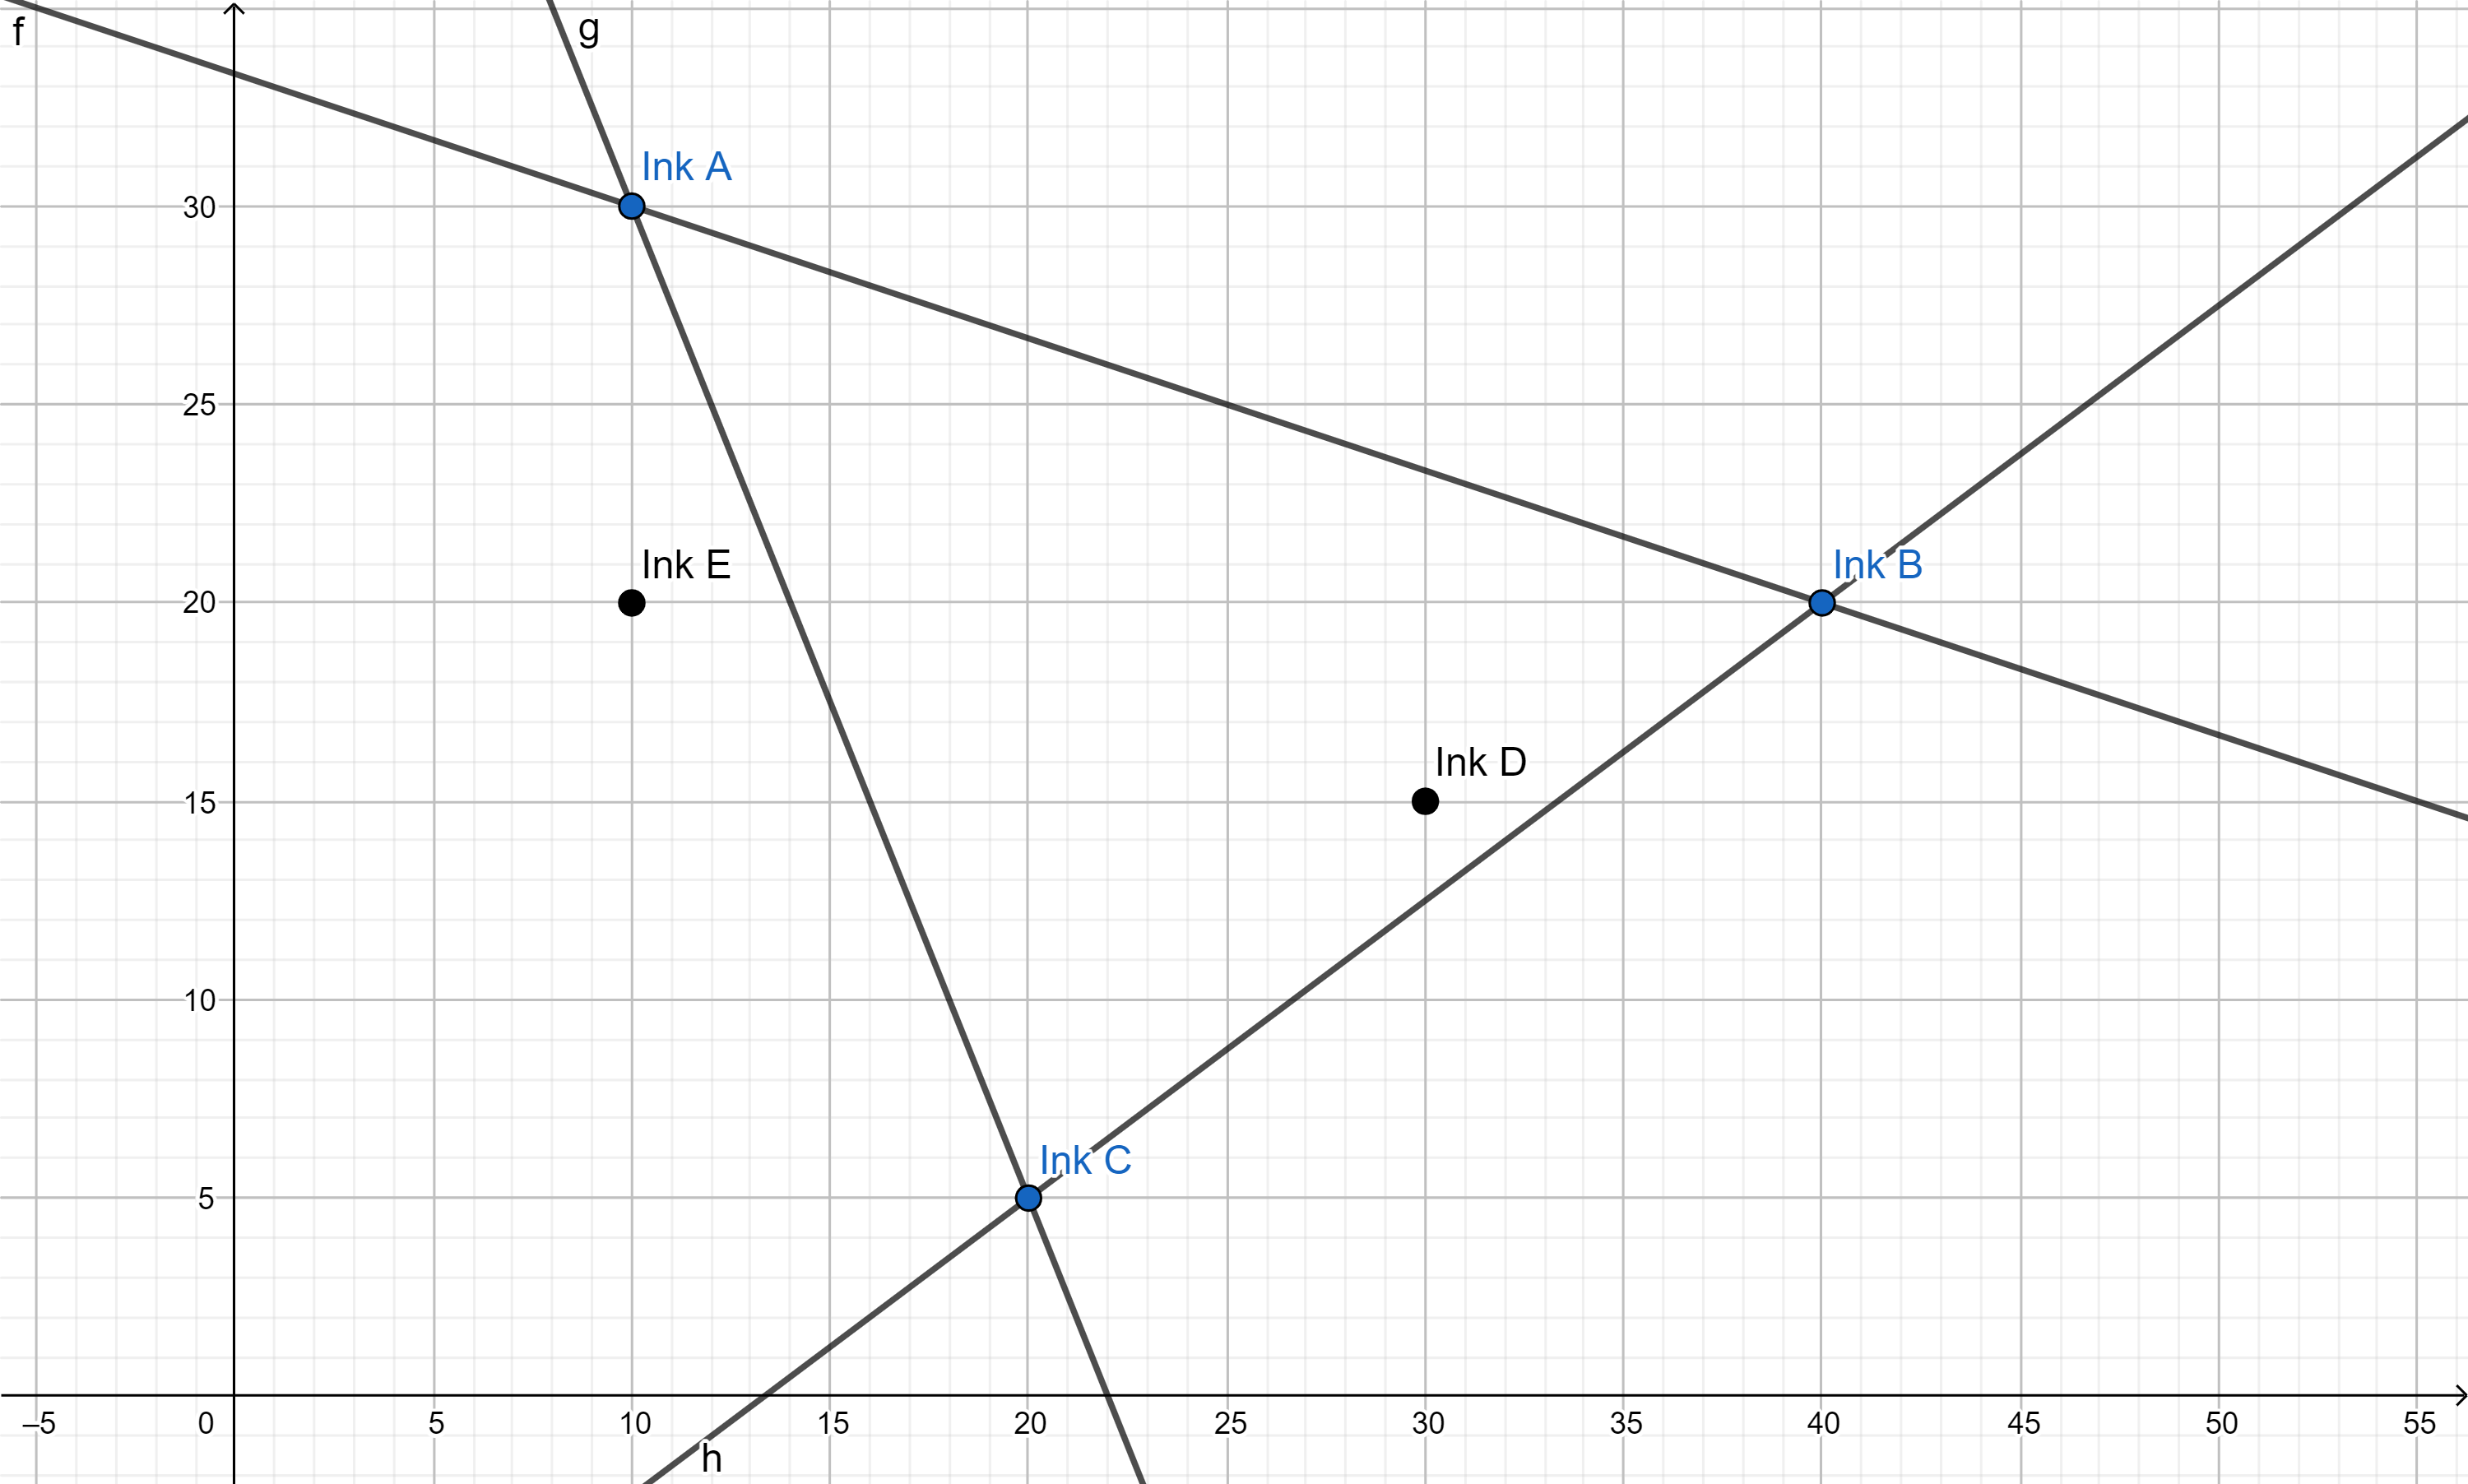
\includegraphics[scale=0.1]{presentation/convex_hull_intro.png}
        \end{figure}
    \end{center}
\end{frame}

\subsection{Problem Definition}
\begin{frame}{What is the Convex Hull Problem?}
    \begin{itemize}
        \item The convex hull problem is formally defined as:
        \begin{center}
            Given a set $S$ of $N$ points in $E^d$, construct its convex hull \textsc{CH}($S$)
        \end{center}
    \end{itemize}    
\end{frame}

\begin{frame}{Lower Bound on Computational Complexity}
    
\end{frame}



% \begin{frame}{Convex Hull in 2D \& 3D}
%   \begin{itemize}
%       \item The smallest convex polygon in 2D or polytope in 3d which encloses a set of points such that each point in the set lies within the polygon/polytope or on its perimeter/faces.
      
%   \end{itemize}
% \end{frame}

\subsection{Algorithms \& Complexities}
\begin{frame}
  \frametitle{Algorithms}
  \begin{itemize}
      \item 2 Dimensional
           \begin{itemize}
               \item Jarvis March
               \item Graham's Scan
           \end{itemize}
      \item 3 Dimensional 
            \begin{itemize}
                \item 
            \end{itemize}
  \end{itemize}
\end{frame}

\begin{frame}
    \frametitle{Jarvis March}
    \lstinputlisting[language=Python,basicstyle=\tiny]{pseudocode/jarvis_march_pseu.py}
    \begin{center}
    $\mathcal{O}(nh)$
    \end{center}
\end{frame}

\begin{frame}{Jarvis March}
     \animategraphics[loop,controls,width=\linewidth,height=200pt]{40}{jarvis_march/jarvis_march-}{0}{190}
\end{frame}


\begin{frame}
    \frametitle{Graham Scan}
    \lstinputlisting[language=Python,basicstyle=\tiny]{pseudocode/graham_scan_pseu.py}
    \begin{center}
    
        $\mathcal{O}(n log n)$
    \end{center}
\end{frame}

\begin{frame}{Graham Scan}
    \begin{center}
        \animategraphics[loop,controls,width=250,height=150pt]{40}{graham_scan/graham_scan-}{0}{50}
    \end{center}
\end{frame}


\begin{frame}
    \frametitle{Chan's Algorithm}
    \lstinputlisting[language=Python,basicstyle=\tiny]{pseudocode/graham_scan_pseu.py}
    \begin{center}
    
        $\mathcal{O}(n log n)$
    \end{center}
\end{frame}

\begin{frame}{Chan's Algorithm}
\begin{center}
      \animategraphics[loop,controls,width=250,height=150pt]{40}{chan_algo/chan_algo-}{0}{50}
\end{center}
\end{frame}


\begin{frame}
    \frametitle{Jarvis March in 3D}
    \lstinputlisting[language=Python,basicstyle=\tiny]{pseudocode/graham_scan_pseu.py}
    \begin{center}
    
        $\mathcal{O}(n log n)$
    \end{center}
\end{frame}



% \appendix
% \section<presentation>*{\appendixname}
% \subsection<presentation>*{For Further Reading}

% \begin{frame}[allowframebreaks]
%   \frametitle<presentation>{For Further Reading}
    
%   \begin{thebibliography}{10}
    
%   \beamertemplatebookbibitems
%   % Start with overview books.

%   \bibitem{Author1990}
%     A.~Author.
%     \newblock {\em Handbook of Everything}.
%     \newblock Some Press, 1990.
 
    
%   \beamertemplatearticlebibitems
%   % Followed by interesting articles. Keep the list short. 

%   \bibitem{Someone2000}
%     S.~Someone.
%     \newblock On this and that.
%     \newblock {\em Journal of This and That}, 2(1):50--100,
%     2000.
%   \end{thebibliography}
% \end{frame}

\end{document}


